\documentclass[english,notitlepage]{revtex4}  % defines the basic parameters of the document
%For preview: skriv i terminal: latexmk -pdf -pvc filnavn


% if you want a single-column, remove reprint

% allows special characters (including æøå)
\usepackage[utf8]{inputenc}
%\usepackage[english]{babel}

%% note that you may need to download some of these packages manually, it depends on your setup.
%% I recommend downloading TeXMaker, because it includes a large library of the most common packages.

\usepackage{physics,amssymb}  % mathematical symbols (physics imports amsmath)
\include{amsmath}
\usepackage{graphicx}         % include graphics such as plots
\usepackage{xcolor}           % set colors
\usepackage{hyperref}         % automagic cross-referencing (this is GODLIKE)
\usepackage{listings}         % display code
\usepackage{subfigure}        % imports a lot of cool and useful figure commands
\usepackage{float}
%\usepackage[section]{placeins}
\usepackage{algorithm}
\usepackage[noend]{algpseudocode}
\usepackage{subfigure}
\usepackage{tikz}
\usetikzlibrary{quantikz}
% defines the color of hyperref objects
% Blending two colors:  blue!80!black  =  80% blue and 20% black
\hypersetup{ % this is just my personal choice, feel free to change things
    colorlinks,
    linkcolor={red!50!black},
    citecolor={blue!50!black},
    urlcolor={blue!80!black}}

%% Defines the style of the programming listing
%% This is actually my personal template, go ahead and change stuff if you want



%% USEFUL LINKS:
%%
%%   UiO LaTeX guides:        https://www.mn.uio.no/ifi/tjenester/it/hjelp/latex/
%%   mathematics:             https://en.wikibooks.org/wiki/LaTeX/Mathematics

%%   PHYSICS !                https://mirror.hmc.edu/ctan/macros/latex/contrib/physics/physics.pdf

%%   the basics of Tikz:       https://en.wikibooks.org/wiki/LaTeX/PGF/Tikz
%%   all the colors!:          https://en.wikibooks.org/wiki/LaTeX/Colors
%%   how to draw tables:       https://en.wikibooks.org/wiki/LaTeX/Tables
%%   code listing styles:      https://en.wikibooks.org/wiki/LaTeX/Source_Code_Listings
%%   \includegraphics          https://en.wikibooks.org/wiki/LaTeX/Importing_Graphics
%%   learn more about figures  https://en.wikibooks.org/wiki/LaTeX/Floats,_Figures_and_Captions
%%   automagic bibliography:   https://en.wikibooks.org/wiki/LaTeX/Bibliography_Management  (this one is kinda difficult the first time)
%%   REVTeX Guide:             http://www.physics.csbsju.edu/370/papers/Journal_Style_Manuals/auguide4-1.pdf
%%
%%   (this document is of class "revtex4-1", the REVTeX Guide explains how the class works)


%% CREATING THE .pdf FILE USING LINUX IN THE TERMINAL
%%
%% [terminal]$ pdflatex template.tex
%%
%% Run the command twice, always.
%% If you want to use \footnote, you need to run these commands (IN THIS SPECIFIC ORDER)
%%
%% [terminal]$ pdflatex template.tex
%% [terminal]$ bibtex template
%% [terminal]$ pdflatex template.tex
%% [terminal]$ pdflatex template.tex
%%
%% Don't ask me why, I don't know.

\begin{document}

\title{FYS 3150 Project 1}      % self-explanatory
\author{Amund Bremer}          % self-explanatory
\date{\today}                             % self-explanatory

\noaffiliation                            % ignore this, but keep it.


\maketitle   
\textit{List a link to your github repository here!}
    
\section*{Problem 1}
Given
\begin{equation*}
    u(x) = 1 - (1 - e^{-10}) x - e^{-10 x},
\end{equation*}
we find that
\begin{equation*}
    u'(x) = (1 - e^{-10})  - (-10) e^{-10 x},
\end{equation*}
and
\begin{equation*}
    u''(x) =  -100 e^{-10 x}.
\end{equation*}
With the supplied source term $f(c)$ given by
\begin{equation*}
    f(x) = 100  e^{-10 x},
\end{equation*}
we get 
\begin{equation*}
    u''(x) =  -f(x).
\end{equation*}
The above is valid for $x \in [0, 1]$, and the boundary conditions $u(0) = u(1) = 0$ are satisfied. Hence, $u(x)$ is an 
exact solution to the given problem.
%
\section*{Problem 2}
A simple c++ script to dump $u(x_i)$ for $x = ih$ is supplied in the file \texttt{main\_2.cpp}, and is plotted in the file 
\texttt{plot\_2.py}. 
\begin{figure}%[h!]
    \centering %Centers the figure
    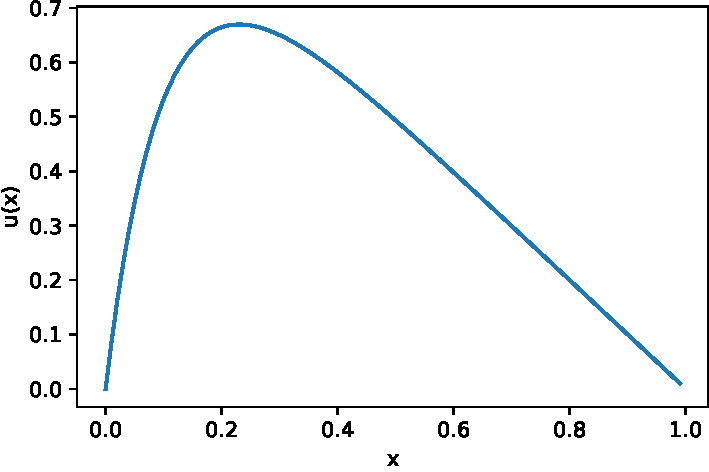
\includegraphics{figs/problem_2.pdf} %Imports the figure.
    \caption{The exact solution $u(x)$ to the Poisson equation with the given source term over its domain.}
    \label{fig:exact}
\end{figure}
%
\section*{Problem 3}
It is well established that an approximation to $u''(x)$ is given as follows:
\begin{equation*}
    u''(x) \approx =  \frac{u(x + h) - 2 u(x) + u(x -h)}{h^2},
\end{equation*}
where $h$ is an appropriately chosen small step-size. For the problem at hand, we are interested in approximating $u''$ over the unit interval.
We define $x_i = i / N$, discretizing the unit interval into $N$ non-overlapping intervals, and let $i = 0 \ldots N$. Furthermore, we 
introduce $u(x_i) = u_i$, and $f(x_i) = f_i$.

Thus, from the original Poisson equation, we can write 
\begin{eqnarray*}
     - \frac{u_{i+1} - 2 u_i + u_{i-1}}{h^2} + \mbox{higher order terms}  & = & f_i, \quad i = 1,\ldots N-1. \\
\end{eqnarray*}
This leads to the simple discrete approxmation $v_i$:
\begin{equation*}
    - (v_{i+1} - 2 v_i + v_{i-1})  = h^2 f_i, \quad i = 1,\ldots N-1. 
\end{equation*}
Here, $v_0 = u_0 = u(0) = 0$, $v_N = u_N = u(1) = 0$, and $h = 1/N$. This is the discrete version of the original Poisson equation, 
and if this is solvable (it is!), we have found approximation to $u(x)$ on the discrete grid $x_i$.
%
\section*{Problem 4}
The discrete equation above

Next up is a table, created using the \texttt{table} and \texttt{tabular} environments. We refer to it by table \ref{tab:output_table}.
\begin{table}%[h!]
    \centering
    \begin{tabular}{c@{\hspace{1cm}} c}
        \hline
        Number of points & Output \\
        \hline
        10 &  0.3086\\
        100 &  0.2550\\
        \hline
    \end{tabular}\caption{Write a descriptive caption here, explaining the content of your table.}\label{tab:output_table}
\end{table}

Finally, we can list algorithms by using the \texttt{algorithm} environment, as demonstrated here for algorithm \ref{algo:midpoint_rule}.
\begin{algorithm}[H]
    \caption{Some algorithm}\label{algo:midpoint_rule}
    \begin{algorithmic}
        \State Some maths, e.g $f(x) = x^2$.  \Comment{Here's a comment}
        \For{$i = 0, 1, ..., n-1$}
        \State Do something here 
        \EndFor
        \While{Some condition}
        \State Do something more here 
        \EndWhile
        \State Maybe even some more math here, e.g $\int_0^1 f(x) \dd x$
    \end{algorithmic}
\end{algorithm}
   
\end{document}

